\section{Core}
The core module extends the JavaScript language with various new features and helper functions. Due to its prototypical nature, the core JavaScript language is easily and naturally extended. The extensions fall in the following categories:

\begin{itemize}
\item Array extensions
\item Object extensions
\item Function extensions
\item Mathematics extensions
\item Support for getter and setter properties
\item Functional pattern matching
\end{itemize}

\subsection{Array Extensions}
The Array prototype is extended in two ways: support JavaScript's version 1.6 and 1.8 so-called array extra's \cite{mozilla07, mozilla08}, and a set of additional helper functions to deal with common array operations. The array extra's includes functions like: \code{forEach}, \code{map}, \code{reduce} (equal to \code{foldr} and \code{foldl} functionality in functional programming languages), \code{filter}, \code{every}, \code{some}, and several other methods. The array extra functions are new---but unofficial---extensions to the JavaScript language defined by the Mozilla developers. Nevertheless these functions have wide support in browsers such as Firefox, Opera, Chrome and Safari. Unfortunately, Internet Explorer does not support them. The core array extra module implements these functions in pure JavaScript and adds them to the Array prototype if they are not already natively supported. This enables the use of the Array extra methods in all browsers.

An example of how this improves clarity follows:
\begin{verbatim}
  function add(a, b) {
    return a + b;
  }

  [1, 2, 4, 1, 6, 5].reduce(add, 0); // returns 19
\end{verbatim}
Without Array Extra's this would have to be implemented using a for loop and accumulation variable.

The additional helper functions included are methods that are strangely omitted from the JavaScript specification, such as a \code{peek} function (\code{pop} and \code{push} are available), contains (to check if an array contains a value), and an \code{isEmpty} method to test for empty arrays.

\subsection{Object Extensions}
In contrast to the other extension modules, the object module does not extend the \code{Object} prototype, which is considered bad practice \cite{arvidsson05}. Instead the module extends the the global \code{Object} object. The consequence is that methods in the extension module should be called with an Object prefix and have the object they operate on passed in as the first argument.

So instead of:
\begin{verbatim}
  obj.someMethod();
\end{verbatim}
We will need to write:
\begin{verbatim}
  Object.someMethod(obj);
\end{verbatim}

The most important function in the object module is \code{extends}, which takes in two or more objects and copies all properties from the second (or third, fourth, etc. depending on how many arguments were passed in as arguments) to the first object. If there is a conflict in property names (i.e. the objects have one or more property names in common) it is first checked if the original property is a built-in property in which case it is kept, otherwise it is overwritten by the last property of that name. The \code{extends} function is used extensively to extend the properties and prototypes of other objects.

The Array Extra's functions are very useful in dealing with arrays. Unfortunately they do not work transparently on objects. For that reason, the object module introduces the same methods contained in the Array Extra's but tailored to deal with objects. This means that functions such as \code{forEach}, \code{map}, \code{reduce}, \code{filter}, \code{every}, and \code{some} can also be used on objects. The functionality and interface is identical to the Array Extra's.

Other functions added to the global Object are designed for more accurate type checking. Although JavaScript is dynamically typed, it is sometimes useful to check for the type of a variable, as the builtin \code{typeof} has some rather severe problems\footnote{For example \code{typeof Array} returns \code{object}.}. There are functions for checking the types of: atoms, numbers, strings, booleans, arrays, and functions. Combined with the array or object extra extensions, it makes it very easy to do input validation. For example, to check if all values in an array are of the type \code{number} we can just write:
\begin{verbatim}
  // returns false (third argument is a string)
  [1, 2, '3'].every(Object.isNumber);
\end{verbatim}
If this is a common desire, we could also add a new function by extending the Array prototype and currying the \code{every} method with the \code{Object.isNumber} method.
\begin{verbatim}
  Object.extend(Array.prototype, {
    isNumber: this.every.curry(Object.isNumber)
  });

  // this now works (still returns false)
  [1, 2, '3'].isNumber();
\end{verbatim}
It is however recommended to keep the number of extensions to the built-in objects to a minimum to prevent name clashes and other interoperability problems.

\subsection{Function Extensions}
The function module extends the Function prototype with a small number of useful functions. The most notable functions are \code{bind}, \code{curry}, and \code{defaults}. Most of these are self-descriptive, but a short example of each follows.

Usually, object methods in JavaScript have a \code{this} property refering to the instance the method is operating on. The bind method allows binding the \code{this} property of a method to any object. Sometimes it may also be useful to bind a function to an object as in the following case:
\begin{verbatim}
  function print() {
    console.log(this.firstname + " " + this.lastname);
  }
  var myPrint = print.bind({ firstname: 'Bender', lastname: 'Rodriguez' });
  myPrint(); // prints "Bender Rodriguez"
\end{verbatim}
Given the \code{add} function used in the Array extensions sub chapter:
\begin{verbatim}
  var add1 = add.curry(1);
  add1(3); // returns 4
\end{verbatim}
The \code{defaults} function is similar to \code{curry} except that it only "curries" a function when one or more of the arguments are missing. In effect this adds default values to optional function parameters. For example:
\begin{verbatim}
  var myAdd = add.defaults(1, 1);
  myAdd();     // returns 2
  myAdd(4);    // returns 5
  myAdd(2, 6); // returns 8
\end{verbatim}
\subsection{Mathematics Extensions}
The math module extends the Math prototype with a set of new methods for rounding, generating correct random integers\cite{glassner90}, and measuring number properties such as accuracy, precision and the number of digits.

The math module also implements interval arithmetic \cite{rokne95}. Interval arithmetic is a method to guarantee upper and lower bounds on imprecise calculations. For example, rounding errors often occur in computer arithmetic due to having only limited precision available in computers. Instead of returning a imprecise exact number to a calculation, interval arithmetic returns a interval which contains the solution. The calculation can then be performed again if more precision in the results are required (or less.)

The interval sub module implements a normal arithmetic functions (add, subtract, multiply, etcetera.) as well as sin, logarithms, powers, exponents, and square roots. Additionally it defines a set of helper functions for determining equality of intervals and inclusion tests. An interval is defined in the module as a JavaScript object with a to and from property which represents the lower and upper bound of the interval respectively.

The chart library uses the interval module extensively, for example as data ranges, or in plotting functions. Data plotting using interval arithmetic is described in a later chapter.

\subsection{Getter and Setter Properties}
The property module adds support for adding getter and setter properties to any object. In fact, it acts as a factory for creating functions that add getter and setter properties to objects. A getter and setter property is defined as a method that when called without a parameter returns the value of its property and when called with a parameter to set the value of the property to that value.

This allows developers to define standard properties and mix them into objects that they desire to have those properties. Instead of redefining an often used property many times, it is created once and added to other objects as desired \cite{crockford08}.
\begin{verbatim}
  // create the property name, parameters, and default values
  var addSize = property('size', {
    width: 100,
    height: 100
  });

  // add the property to a new (empty) object
  var myObject = addSize({});

  // returns {width: 100, height: 100}
  myObject.size(); 
  // sets width to 200 and returns {width: 200, height: 100}
  myObject.size({width: 200});
\end{verbatim}
The example also shows that by taking in the "setter" value as an object, the property is not restricted to a fixed number of arguments or the order of arguments.

\subsection{Functional Pattern Matching}
Pattern matching is a form of conditional branching which allows concise matching of data structure patterns and binding variables at the same time \cite{wikipedia09}. Pattern matching is supported in some functional languages such as ML, Haskell, OCaml, and Erlang. This \code{fun} module implements pattern matching for the JavaScript language in an efficient and concise way. The following is an example of pattern matching:
\begin{verbatim}
  var fact = fun(
    [0, function ()  1],
    [$, function (n) n * fact(n - 1)]
  );
\end{verbatim}
The above function implements a simple factorial function using the \code{fun} module. When \code{fact(10)} is called the value \code{10} is matched against the first pattern \code{0}. This match fails and the next pattern is evaluated. The ‘\$’ in the next pattern is an example of a parameter. A parameter matches anything, so the match succeeds and \code{10} is passed as an argument to the anonymous function. Since this is a recursive function it will match the second pattern until the argument to the function reaches zero and then terminates. Note that this example uses JavaScript 1.8 syntax, code in previous JavaScript versions will be slightly more verbose.

Another common use of pattern matching is to determine if a value is of a certain type and perform an action depending on the result. For example, say we have a \code{print} function which logs its value to the console. We would however like to customize the output for some data types. We can accomplish this using pattern matching as follows:
\begin{verbatim}
  var print = fun(
    // match and return Date values
    [Date, function (d) ...],

    // match and return String values
    [String, function (str) ...],

    // match and return any other type
    [$, function (o) ...]
  );
\end{verbatim}
If the type of the value is Date, the first anonymous function will be executed and its value passed as argument. The same applies to values of type String. Any other value will be passed to the last anonymous function whose pattern acts as a catch-all. 

\subsubsection{Object extraction}
Patterns can also contain wildcards, which can be used to ‘mask out’ or ignore certain parts of the value it is matched against. This can be used to concisely extract properties for large and deeply nested objects. For example:
\begin{verbatim}
  var data = {
    label: 'Plot #1',
    type: 'points',
    values: [2.1, 5.6, 2.4, 3.4]
  };

  var parse = fun(
    [{label: _, type: _, values: $}, function (v) console.log(v)]
  );

  parse(data); // prints out [2.1, 5.6, 2.4, 3.4]
\end{verbatim}
\subsubsection{Algebraic data types}
Pattern matching can also be used with Sjoerd Visscher's Algebraic data type library \cite{visser08}. In the following example we define a simple binary tree data type. The tree can contain either \code{Void} or a \code{Bt} tuple. The tuple consists of a value, and two branches called left and right. In the ML programming language we would define a polymorphic binary tree like this:
\begin{verbatim}
  datatype 'a binarytree = Void | Bt of 'a * 'a binarytree * 'a binarytree
\end{verbatim}
In JavaScript---using the ADT library---it looks like this (note that this binary tree is not polymorphic, its values are numbers.)
\begin{verbatim}
  var BinaryTree = Data(function (binarytree) ({
    Void : {},
    Bt: { v: Number, L: binarytree, R: binarytree }
  }));
\end{verbatim}
We can then create a simple binary tree instance using this definition. A visual representation of this binary tree is shown in Figure \ref{btree}. 
\begin{verbatim}
  var bt = Bt(4, 
      Bt(2, Bt(1,Void,Void), 
            Bt(3,Void,Void)), 
      Bt(8, Bt(6, Bt(5,Void,Void), 
                  Bt(7,Void,Void)), 
            Bt(9,Void,Void)));
\end{verbatim}

\begin{figure}[h!]
\centering
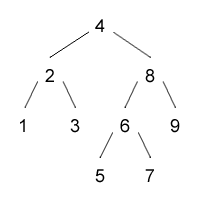
\includegraphics[width=.3\linewidth]{btree}
\caption{Binary tree}
\label{btree}
\end{figure}

We can now define various functions, for example to calculate the number of leafs (nodes without children) in the tree, or a function to test whether a value is a member of the binary tree. It is possible to use the data types in patterns, for example the \code{numLeafs} method first matches on an empty node, then a leaf node and finally on any other kind of node. The \code{isMember} method shows that the matching is not limited to one function parameter; the value to search for is taken as the first parameter and the binary tree as the second parameter.
\begin{verbatim}
  var numLeafs = fun(
    [Void, function() 0],              // empty node
    [Bt(_, Void, Void), function() 1], // leaf node
    [Bt(_, $, $), function(L, R) numLeafs(L) + numLeafs(R)]
  );

  var isMember = fun(
    [_, Void, function() false],
    [$, Bt($, $, $), function(x, v, L, R) x === v || 
	  (isMember(x, L) || 
       isMember(x, R))
    ]
  );

  numLeafs(bt);     // 5
  isMember(10, bt); // false
  isMember(3, bt);  // true
\end{verbatim}
The following two functions return a list of all the elements using in order and pre order traversals of the binary tree.
\begin{verbatim}
  var inorder = fun(
    [Void, function() []],
    [Bt($, $, $), function(v, L, R) inorder(L).concat([v], inorder(R))]
  );

  var preorder = fun(
   [Void, function() []],
   [Bt($, $, $), function(v, L, R) [v].concat(preorder(L), preorder(R))]
  );

  inorder(bt);      // [1,2,3,4,5,6,7,8,9]
  preorder(bt);     // [4,2,1,3,8,6,5,7,9]
\end{verbatim}
A real implementation of a binary tree would of course not use the data types and functions defined in this article for performance reasons, but a binary tree serves as a good introduction to both pattern matching and algebraic data types in JavaScript.
